%!TEX root = paper.tex
%%%%%%%%%%%%%%%%%%%%%%%%%%%%%%%%%%%%%%%%%%%%%%%%%%%%%%%%%%%%%%%%%%%%%%%%%%%%%%%%
\section{An End-to-End Lag Model}
\label{sec:model}

It is evident from the discussion in Section~\ref{sec:background} that multiple different components contribute to the end-to-end lag in games, and that multiple potential models and levels of granularity exist for each game type. Let's discuss therefore the model boundaries and level of detail used in the current iteration of this analytical model to be presented here.


\begin{table}[!t]
\caption{Notation used in the model. Random variables are denoted by capital letters $X$, and constants by small letters $x$.}
\label{tab:notation}
	\centering
	\begin{tabu}{lX[1,l]X[1,l]}
	\toprule
	\textbf{Symbol} & \textbf{Description} & \textbf{Simulation} \\
	\midrule
	$D$ & network delay between game client and server & $D \sim TNorm(\mu_D;\sigma_D)$, $\mu_D = \SI{20}{\milli\second}$; $\sigma_D = \SI{5}{\milli\second}$\\
	$P$ & game server processing time & $P \sim TNorm(\mu_P;\sigma_P)$, $ \mu_P = \SI{3}{\milli\second}; \sigma_P = \SI{0.1}{\milli\second}$\\
	$T$ & end-to-end lag & key performance measure \\
	$U$ & (inter arrival) time between user inputs & $U \sim Exp(\lambda)$; $\lambda = \SI{50}{\milli\second}$\\
	\midrule
	$c$ & command rate & $c=g$ \\
	$c^{-1}$ & interval to gather input events before sending & \\
	$d$ & decode delay & \SI{5}{\milli\second} \\
	$e$ & encode delay & \SI{15}{\milli\second} \\
	$f$ & framerate & $f \in \SIrange{10}{200}{\hertz}$ \\
	$f^{-1}$ & frame duration & $f^{-1} \in \SIrange{5}{100}{\milli\second}$ \\
	$g$ & game tickrate & $g \in \SIrange{10}{200}{\hertz}$ \\
	$g^{-1}$ & game tick duration & $g^{-1} \in \SIrange{5}{100}{\milli\second}$ \\
	\bottomrule
	\end{tabu}
\end{table}

\subsection{Model of end-to-end lag for online games}
%\hoss{Ich wuerde mathematische Notation einfuehren, um klar zu machen, was Teil des Modells ist.}
First, we define the end-to-end lag $T$ to be the time elapsed from when the player supplies commands to the input devices until just before actual audio/video output.
% I.e.: rendering, *and* encode/decode for cloud games
We assume that the actual presentation of audio and video content happens instantaneously (ignoring any screen synchronization issues), and assume the player input to be a stochastic process $U$. % future work!1!!
Furthermore, as also found in practice, input events are queued up and sent en bloc at specific intervals defined by the command rate $c$.

Second, in our treatment of client-server games, we focus on modeling a single connected client and its interaction with the game server. While other clients might be connected to the same server, it is solely the server that controls when game state updates are sent. Thus, the client we are looking at does not need to account for the behavior of other clients.
% probaby not future work

Next, we associate a static (but individually configurable) tick rate $g$ with the computation process of the game server, and a frame rate $f$ with the render process. The server updates the state of the game world at every tick, and may spend some processing time $P$ in order to do so. The processing time is a random variable which is assumed to follow a truncated normal distribution in our simulations. Once finished, an update message is sent to the client. Since the client needs time to render this update, it is displayed only after the next, upcoming frame. Independent of the update process, the game client outputs the next video frame in accordance to the frame rate. The game client's state might not get updated by the server between rendered frames. Still, output is generated\footnote{A practical game implementation will use state prediction for this.}. The round-trip to the server and back implies that the lag between an input event and the earliest frame containing a perceptible result of that event can take multiple frame times.

While we consider the command, tick, and frame rates to be constant (though not necessarily identical), there is no inherent synchronization between them. This is represented in the simulation by a random initial phase offset for each rate.

Finally, since we are simulating online games, the simulation obviously includes the network paths between the different components. The delay distributions are freely configurable, but may be omitted entirely as well. We assume a random variable $D$ representing the networking delay between game client and server. Fig.~\ref{fig:queuing-model} gives a graphical representation of the queueing model for the online video game case, especially including the three clocked processes responsible for the game's interactions.
%\hoss{Explanation of Figure~\ref{fig:queuing-model} is missing. What is the meaning of the other queues? Mit der Tabelle~\ref{tab:notation} und Update von Fig.~\ref{fig:queuing-model} sollte das klarer werden.}
Moreover, Fig.~\ref{fig:tickrate-timeseries} shows the flow of events between game client and server for the simplified case of an online video game.

\begin{figure*}[!t]
	\centering
	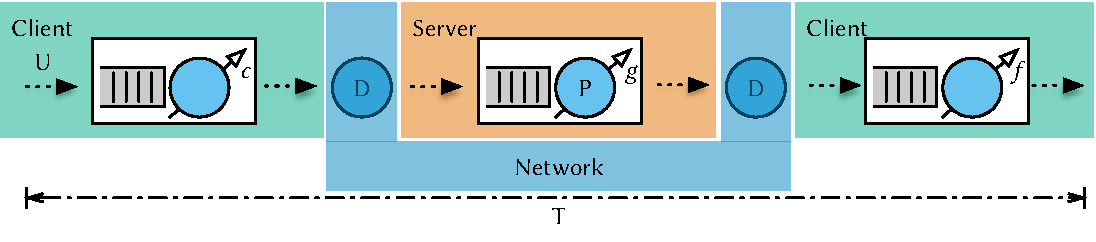
\includegraphics[width=1.0\textwidth]{../../models/e2e-lag-model.pdf}
	\caption{Abstract end-to-end lag queuing model representation in the online video game case. The clock rate is denoted in the top right corner of each process. See Tab.~\ref{tab:notation} for the notations.
	%\hoss{Die Queues sind nicht ganz korrekt so. Es werden periodisch alle Events verarbeitet und weitergereicht. Hier sieht es nach FIFO und Einzelabarbeitung aus. Ausserdem sind die Variablen $N_C$ usw. nicht erklaert. Ausserdem wird im Model nicht erklaert, dass es einen Gaming Processing Delay am Game Server gibt.}
	}
\label{fig:queuing-model}
%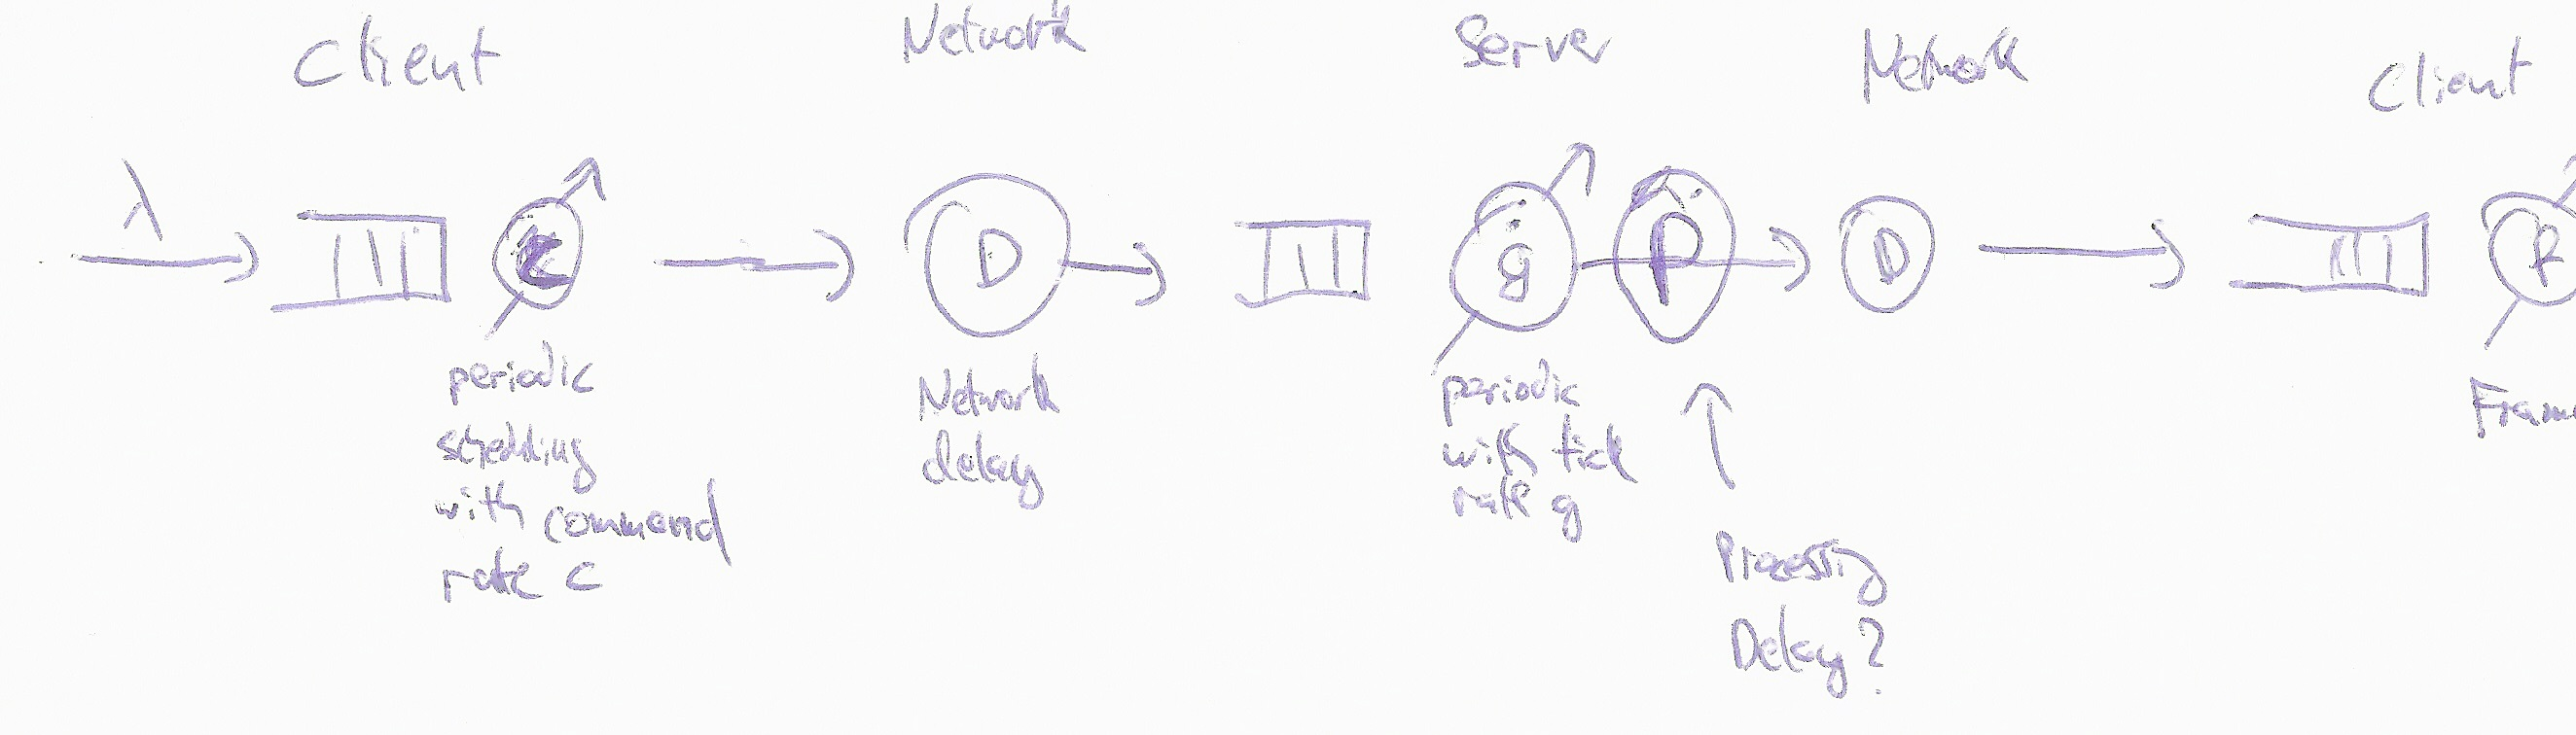
\includegraphics[width=0.8\textwidth]{figure7-queueingModel.jpg}
%\caption*{\hoss{Wie waere es, ein Symbol einzufuehren, dass den periodic Update mit entsprechender Rate zeigt?}}
\end{figure*}


\begin{figure}[!t]
	\centering
	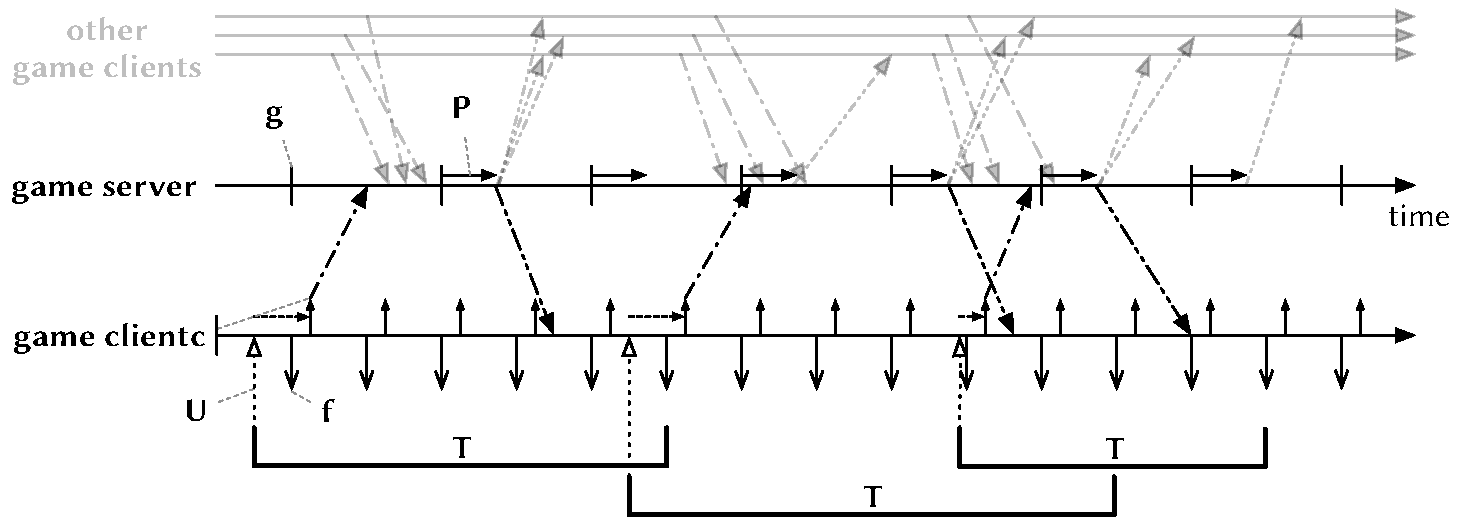
\includegraphics[width=1.0\columnwidth]{../../models/tickrate-timeseries-notation.pdf}
	\caption{Exemplary flow of events in an online client-server game, and resulting end-to-end lag with the notation of Tab.~\ref{tab:notation}.
	% \hoss{Notation aus Tabelle ~\ref{tab:notation} waere gut im Bild. }
	} %Delay values are given for a framerate of \SI{60}{\hertz} and a server tickrate of \SI{30}{\hertz}, the network latency will only show minor variations.}
\label{fig:tickrate-timeseries}
\end{figure}



\subsection{Model of end-to-end lag for cloud games}
The model for cloud gaming (Fig.~\ref{fig:component-models}c) is based on the online game model, adapting its notions of $D$, $P$, $T$, $U$, $c$, and $f$. However, the server now handles only one client, and becomes a \textit{streaming server} that also renders and encodes the screen contents, adding a constant encoding delay $e$. On the client side, the stream is decoded (adding decoding delay $d$) before being displayed.



\subsection{Model Simplifications}

These simulation models do not attempt to capture all possible sources of lag that. Indeed, we simplify the models in the following aspects in the hope to make the results more tractable.
%\textbf{TODO Make this more of a ``future work'' section, less ``why we suck''.}

\myparagraph{Additional delay sources}
The models ignore the delays contributed by input devices like keyboards, mice, and game controllers. We estimate these at below \SI{10}{\milli\second}. The same goes for the lag of the display device (from after rendering or decoding until the frame is actually visible) which is typically in the range of 1--3 frame times for a computer monitor, and larger for TV sets. The models can be extended to take those delay factors into account, but they were exempted for the sake of simplicity in this paper.
% TODO: \textbf{Add adaptive VSYNC?}

\myparagraph{Subtleties of game internals}
Modern games go great lengths to handle lag gracefully, and try to ``work around it'' in various ways. The methods for this vary, and implementations usually are not open for examination, so we leave them for further study. Techniques include lag compensation (the game client tries to predict the server state from past knowledge, allowing for smoother local updates but possibly causing slight deviation and re-synchronization artifacts), and tick- and framerate adaptation at the game server and client, respectively. Lastly, player actions in a game might take multiple command time intervals to perform. The simulation currently assumes that every single batch of commands that reaches the server will result in state updates and thus changes in the perceptible output of the game client. It should be noted that none of these techniques alter the end-to-end lag itself, rather they just try to conceal it on some higher level. Therefore, the mechanisms do not invalidate our examination.

\myparagraph{Factors in human perception and strategy}
The models we present do not take into account the perceived lag from when the players \textit{think} they have triggered an action to when they perceive the outcomes of their action. This consequently disregards effects of different player actions, strategies, and so on.




%%%%%%%%%%%%%%%%%%%%%%%%%%%%%%%%%%%%%%%%%%%%%%%%%%%%%%%%%%%%%%%%%%%%%%%%%%%%%%%%
% \subsection{Sources of Latency in Gaming}
% \label{sec:latency}






%All in all, if possible, video game measurements should always consider the full \textbf{end-to-end} lag factoring in every possible source of delay but also the presence latency compensation and concealment techniques.



% Online games attempt to compensate network latency through various means, such as already showing the results of your local inputs while waiting for the authoritative update from the server and potentially rolling back the local updates.

% TODO: Also mention lag compensation/concealment techniques:
% Client-side: non-authoritatively update game state based on own inputs and merging it afterwards with the server's view, correcting any prediction errors
% Server-side: Keep a short history of past game states, and do not execute player commands at the state they were received but rather at the (estimated) state time they were intended for.

% lag compensation can also be implemtented specifically for cloud gaming as the work conducted in \cite{Lee:2015:OUS:2742647.2742656} suggests, however incurring siginficant overhead in terms of processing time for the game logic and renderer as well as the encoding and bandwidth due to specutatively generating and transmitting frames ahead of their corresponding input.


% game keeps history of recent game state snapshots to interpolate between two server states and create a smoother experience (thus decoupling client frame rate from the server's state updates), but adds e.g. \SI{100}{\milli\second} of view lag due to snapshot history.


%%
%\subsubsection{Online Video Game Latency Concealment Techniques}


% input: absolute (eg mouse) vs. relative (analog stick)
% frame perfect input
% double/triple buffering
% inputs per minute vs timing precision of input
% range of interactivity
% latency sensitivity/responsiveness of different game mechanics / UI elements in the same game
% latency of camera movement / UI vs actual game elements


%Info on source engine networking: \url{https://developer.valvesoftware.com/wiki/Source_Multiplayer_Networking}
%\url{https://developer.valvesoftware.com/wiki/Latency_Compensating_Methods_in_Client/Server_In-game_Protocol_Design_and_Optimization}
%(Latency Compensating Methods in Client/Server In-game Protocol Design and Optimization, Yahn W. Bernier (yahn@valvesoftware.com), 2001, Software Development Engineer, Valve Software)



% Online games generally follow one of two designs. Either there is a dedicated server available to host the game, or one of the clients is elected to additionally act as the server.
% The election is typically based on criteria such as the available performance and latency. If the selected host drops out of the game, a new server has to be elected and the game gets migrated there, usually stopping the game for a few moments. Competitive games almost always choose the dedicated approach to ensure fairness, stability and better control cheats.



% \begin{figure*}[!t]
% 	\centering
% 	\begin{subfigure}[b]{0.5\textwidth}
% 		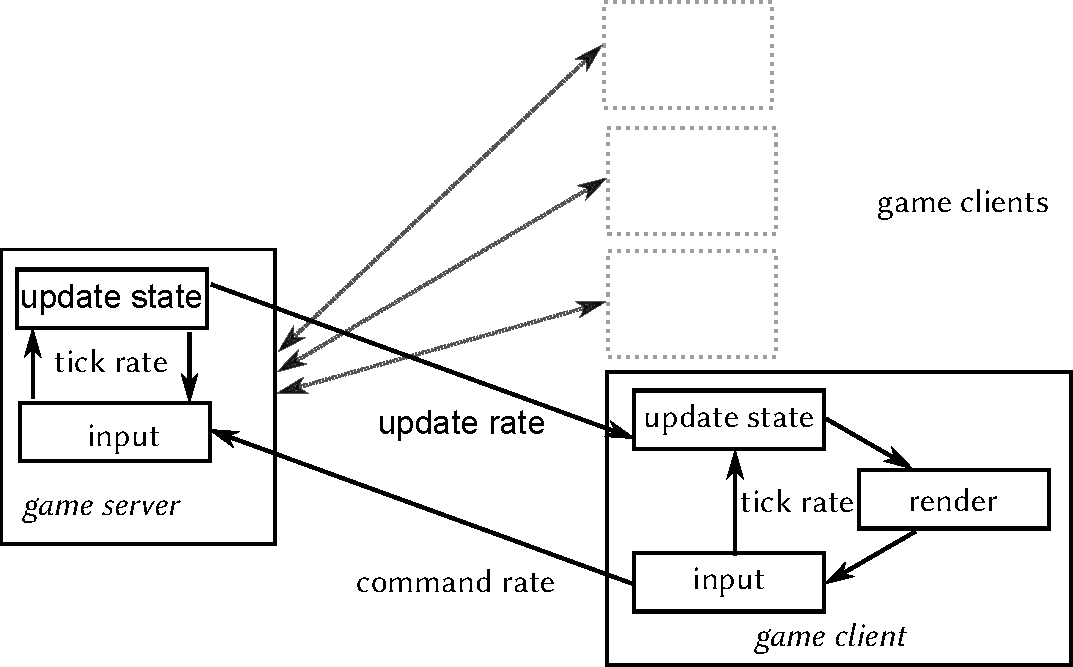
\includegraphics[width=1.0\columnwidth]{images/game-tick-rate.pdf}
% 		\caption{In typical online games.}
% 		\label{fig:tickrate-online}
% 	\end{subfigure}%
% 	~
% 	\begin{subfigure}[b]{0.5\textwidth}
% 		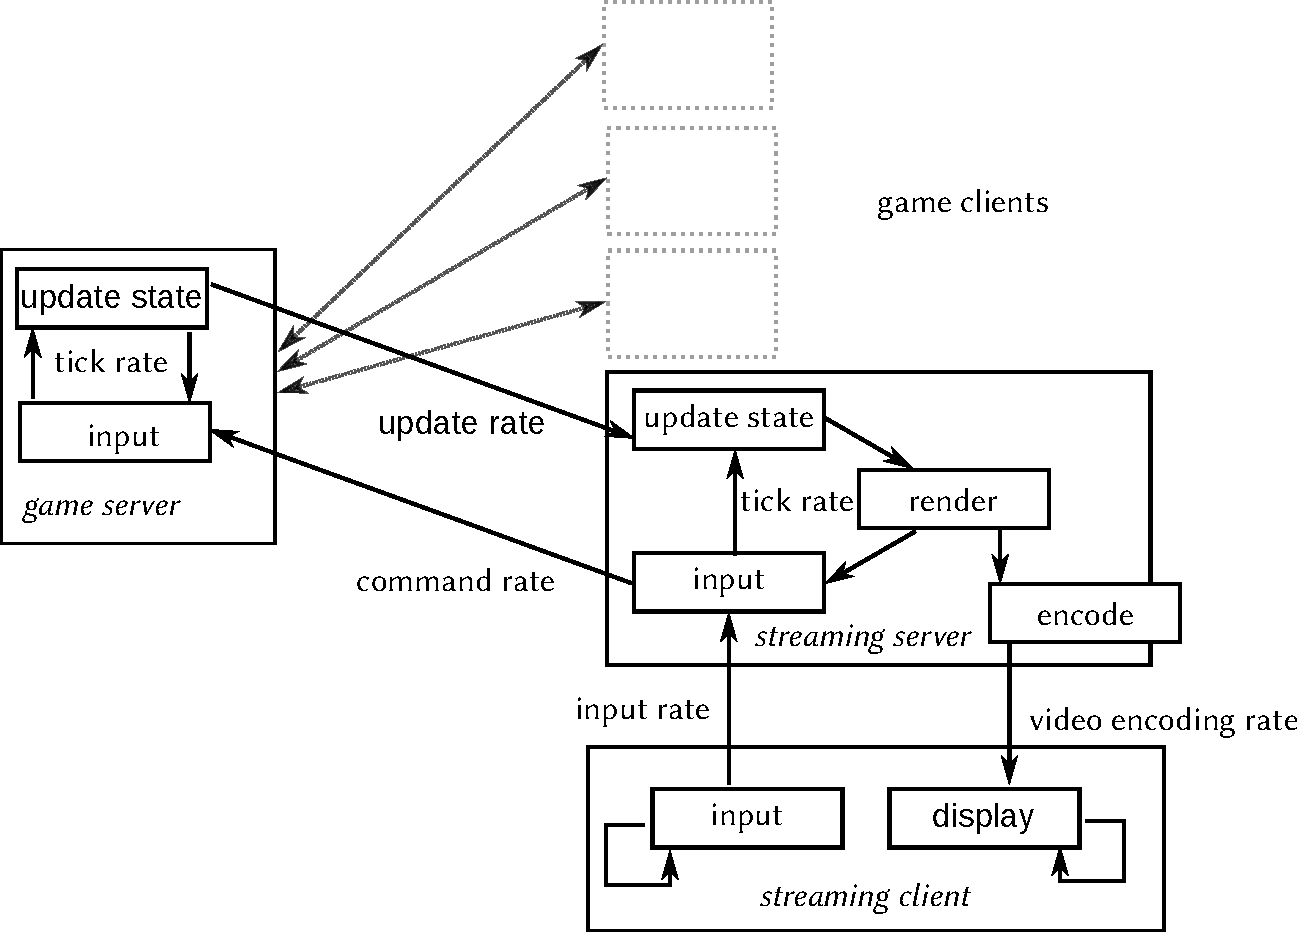
\includegraphics[width=1.0\columnwidth]{images/game-tick-rate-streamed.pdf}
% 		\caption{In a cloud gaming scenario.}
% 		\label{fig:tickrate-streamed}
% 	\end{subfigure}
% 	\caption{Interaction of the game client and server.}
% 	\label{fig:tickrates}
% \end{figure*}



% \begin{figure}[!t]
% 	\centering
% 	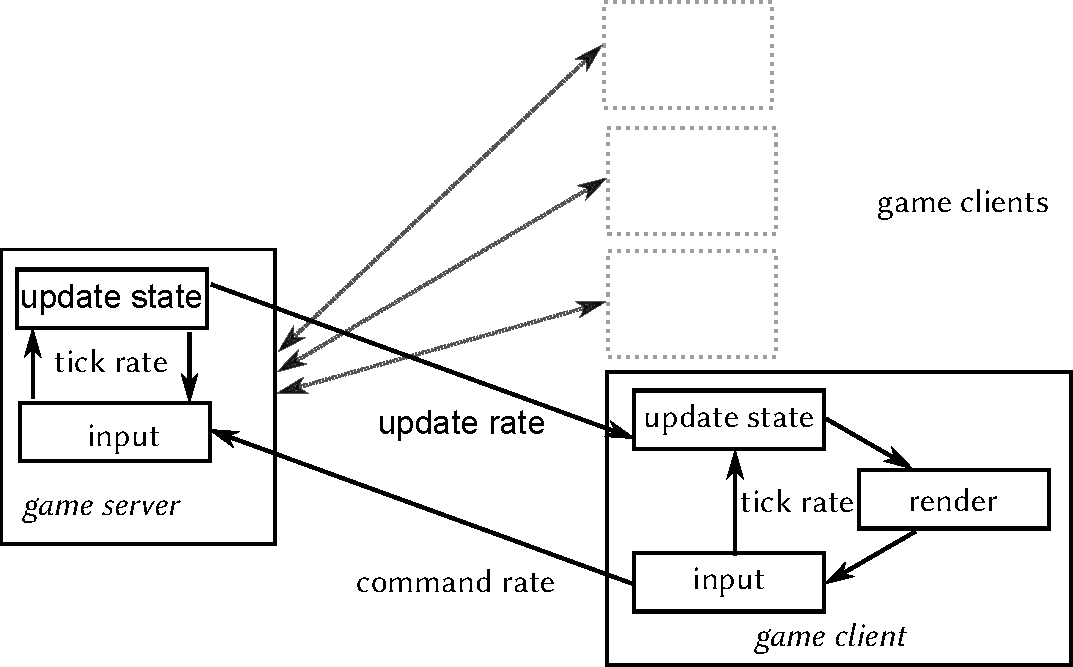
\includegraphics[width=1.0\columnwidth]{images/game-tick-rate.pdf}
% 	\caption{Interaction of client and server in typical online games.}
% \label{fig:tickrate-online}
% \end{figure}








% \subsection{Determining Video Game Popularity and Engagement}
% FUTURE WORK!

% Using Steam data as a popularity measure and get a grasp of which games could be worthwhile to look at. Ties in to user engagement metrics to determine the quality a game delivers in a current situation. Alternative view: the more engaged players are to a game, the more important is delivering a good quality (e.g. for streaming).

% For example, there might be a correlation between a game's price and the average time it's been played, as Figure~\ref{fig:tickrate-streamed}.


% Other  k-means clustering of steam/price data or other graphs

% \begin{figure}[!t]
% 	\centering
% 	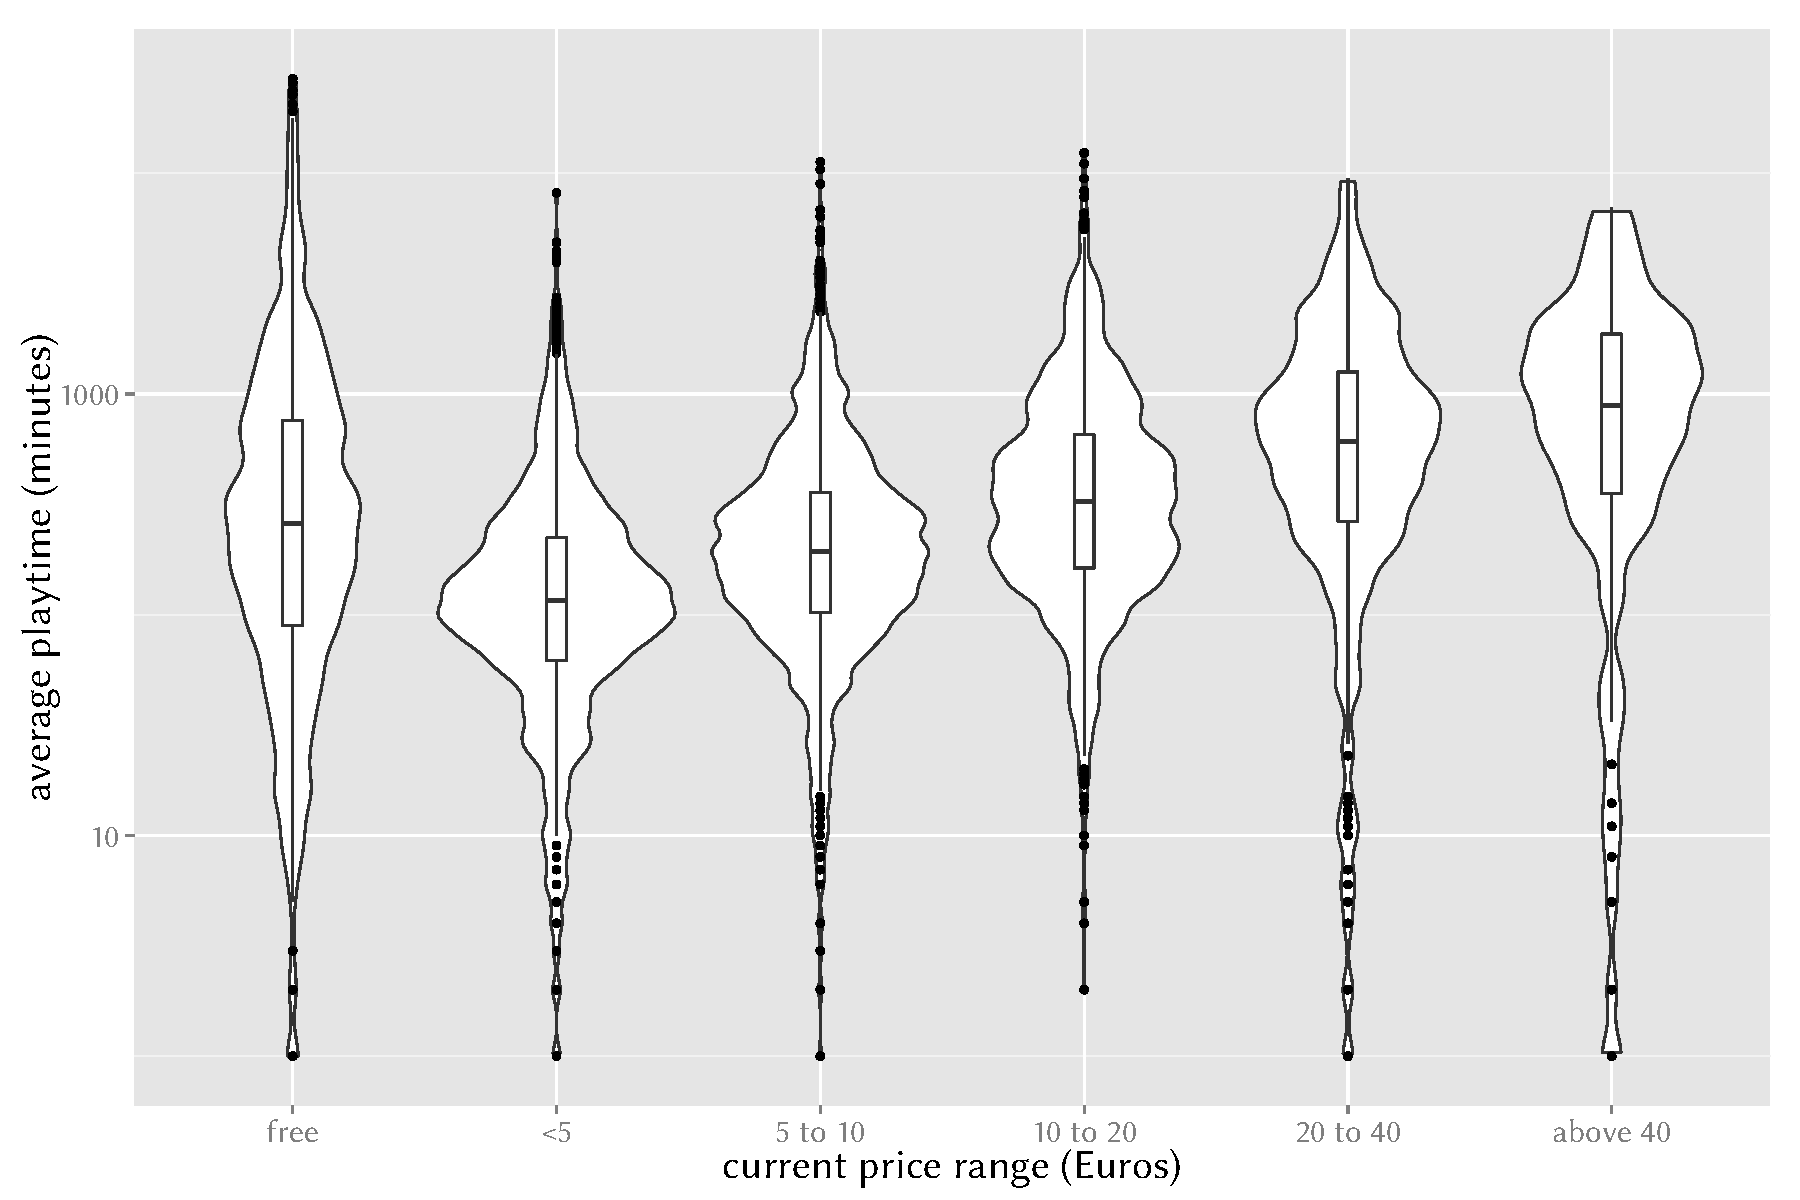
\includegraphics[width=1.0\columnwidth]{images/dampfviolinen-playtime.pdf}
% 	\caption{Game cost as a possible categorization and engagement factor. Displayed is a violin plot of the current costs in relation to the average playtime of individual games.s}
% \label{fig:cost-playtime-violin}
% \end{figure}

% Categorization dimensions viable for measuring online video game quality:



%\footnote{\url{http://accidentalscientist.com/2014/12/why-movies-look-weird-at-48fps-and-games-are-better-at-60fps-and-the-uncanny-valley.html}}
%\url{https://stackoverflow.com/questions/17411/how-do-you-separate-game-logic-from-display}
%\url{http://higherorderfun.com/blog/2010/08/17/understanding-the-game-main-loop/}
